\documentclass{article}
\usepackage[utf8]{inputenc}
\usepackage[top=2.54cm, outer = 2.54cm, inner = 2.54cm]{geometry}
\usepackage{graphicx}
\usepackage{hyperref}
\usepackage{color}
\usepackage{float}
\usepackage{titlesec}     %title formats library
\usepackage{changepage}   %subs library
\usepackage{indentfirst}  %indentation library
\usepackage{newtxmath,newtxtext}    %font library
\usepackage[hang]{footmisc}     %footnote margin library
\usepackage{appendix}     %appendix library
\usepackage[sorting=none]{biblatex}
\bibliography{multi.bib}

%% title format %%
\titleformat*{\section}{\Large\bfseries}
\titleformat*{\subsection}{\large\itshape}
\titleformat*{\subsubsection}{\normalfont\itshape}
\titleformat*{\paragraph}{\large\bfseries}
\titleformat*{\subparagraph}{\large\bfseries}

%% paragraph indentation format %%
\newenvironment{subs}
  {\adjustwidth{3em}{0pt}}
  {\endadjustwidth}

%% footnote margin format %%  
\setlength\footnotemargin{10pt}
  
\title{\textbf{% 
       Multimodal Speech Emotion Recognition Using\\ 
       Audio and Text [Research Replication]}}
\author{Jan Arvin Lapuz, Alyssa Lim, Le Van Nguyen, Ramil Zabala}
\date{}
\begin{document}
\maketitle

\noindent\rule{16.5cm}{0.4pt}\\
    % \\
    \begin{center} \textbf{\large Abstract} \end{center}
    \par
    %% edit par par here. %%
    A few studies have been carried out on developing models that classify emotions out of speech audio but never has dialogue transcript been incorporated to improve accuracy. In 2018, Seunghyun Yoon, et al. conducted a research that introduced a deep dual recurrent encoder model that combines audio features, such as MFCC and prosody, text data to predict the one of the four emotions – angry, happy, sad and neutral. Their model achieved a WAP value of up to 71.8\%. This paper attempted to replicate their results using the original IEMOCAP data and extend it to new datasets. The replication using the original data resulted in an accuracy of within 0.1\% of the published result except for the MDREA model which had 21\% reduction in accuracy. To extend the replicaton, new methodologies have been applied on YouTube videos to suit the model and reached a maximum WAP accuracy of 27\%. Existing audio data such as the TESS dataset was also used with a slightly better maximum WAP accuracy of 31\%.\par 
\noindent\rule{16.5cm}{0.4pt}

\section{Research Description}
    Since this project's purpose is to conduct an extended replication of a reproducible quality research, one paper that adapts these criteria is Multimodal Speech Emotion Recognition Using Audio and Text\cite{yoon2018multimodal}.\par
    
    Many studies have been carried out that aim to create a model classifying emotion from speech. However, those models rely solely on audio features of speech data and does not deliver desired result. In the mentioned paper, Seunghyun Yoon, Seokhyun Byun, and Kyomin Jung introduce a deep dual recurrent encoder model that simultaneously utilises both audio and transcript of speech data. In detail, the raw conversation dialogues and their transcripts are encoded by a dual recurrent neural networks (RNNs) before being combined to predict their emotion category -  happy, sad, angry and neutral. By applying this architecture on the IEMOCAP dataset, the model is able to achieve up to 71.8\% of accuracy.\par

    For comparison, the paper considered four models in total:
    \begin{itemize}
        \item \textbf{Audio Recurrent Encoder(ARE)} utilises audio features only
        \item \textbf{Text Recurrent Encoder(TRE)} utilises text features only
        \item \textbf{Multimodal Dual Recurrent Encoder(MDRE)} utilises audio and text features simultaneously.
        \item \textbf{Multimodal Dual Recurrent Encoder with Attention(MDREA)} utilises audio and text features simultaneously with attention mechanism
    \end{itemize}
    
    The overall performance of the models are measured by the weighted average precision (WAP) value over the 5-fold cross validation data folders\footnote{WAP calculation:\\ \url{https://github.com/david-yoon/multimodal-speech-emotion/blob/master/model/evaluation_text.py}}. With this evaluation framework, the performance of MDRE is reported to have highest WAP in the paper (at around 71.8\%).\par

\begin{subs}
    \subsection{Justification}
        The quality of the paper is demonstrated by the fact that it is published as a part of the 2018 IEEE Spoken Language Technology Workshop (SLT), which is ranked 14th in Computational Linguistics Category on Google Scholar \cite{Google Scholar Computation linguistics}. Furthermore, the paper was cited 58 times at the time of writing of this report\footnote{Papers that cite the research paper in Google Scholar:\\ \url{https://scholar.google.com.au/scholar?cites=16749771682156267984&as_sdt=2005&sciodt=0,5&hl=en}}. Although a pre-trained model is not provided, the paper's source code is available through one of the authors' Github repository\footnote{Author's github repository:  \url{https://github.com/david-yoon/multimodal-speech-emotion}}. 
\end{subs}

\section{Original Dataset Description}
    The original dataset discussed in the paper is from Interactive Emotional Dyadic Motion Capture (IEMOCAP) database\footnote{IEMOCAP database: \url{https://sail.usc.edu/iemocap/}}. It consists of roughly 12 hours of audiovisual data of acted conversations from 12 actors in which only speech (.wav format) and transcript (.txt format) data are selected.\par

    Before inputting into the architecture, some modifications had been made. The audio signal is extracted into Mel-frequency Cepstral Coefficients (MFCCs) and prosodic features using the openSMILE toolkit while the transcript is tokenised and indexed by Natural Language Toolkit(NLTK). The processed data are all in numpy format.\par
    
    After acquiring IEMOCAP database's license agreement, the replication team was able to collect the author's IEMOCAP pre-processed dataset via an application link\footnote{Application to download IEMOCAP pre-processed dataset (SLT-18):\\  \url{https://docs.google.com/forms/d/e/1FAIpQLSdSrvnpoxltYnjq_QcFCl6GXfEco8G5JNEgpFuo56VhPM9Zbg/viewform}}.\par
    
    Figures \ref{fig:Extracted MFCC features} and \ref{fig:Extracted Prosodic features} show snippets of processed MFCC and prosodic features of audio data, respectively.\par
    
    \begin{figure}[H]
        \centering
        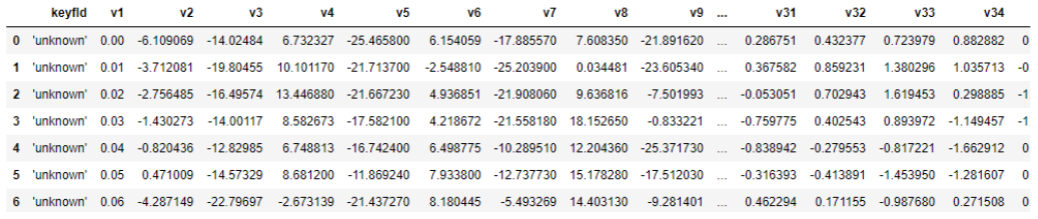
\includegraphics[width=12cm]{Images/mfcc.PNG}
        \caption{Extracted MFCC Features}
        \label{fig:Extracted MFCC features}
    \end{figure}
    
    \begin{figure}[H]
        \centering
        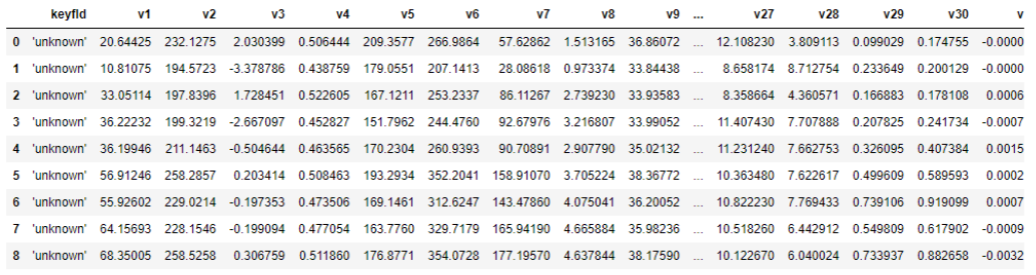
\includegraphics[width=12cm]{Images/prosody.PNG}
        \caption{Extracted Prosodic Features}
        \label{fig:Extracted Prosodic features}
    \end{figure}
    
\section{Replication of Original Work}
    Replications are done to validate the findings of the original work. To execute the replication successfully, first, the replicators must understand the goal of the research. The research proposed a novel deep dual recurrent model, which simultaneously utilise the text data and audio signals to analyze speech data. Original and pre-processed data, tools, and guides were made available by the authors of the original work. The goal of the group is to successfully replicate the proposed model using the original data, then extend the replication to the group's new dataset. In order to do so, the structure of the data used in the original work was carefully studied and reviewed. Familiarization with the approach used in the paper as well as the environment the researchers used, ability to weigh the resources needed, and identification of potential roadblocks in the replication process are also aspects to focus on. The group re-evaluated the overall performance of the proposed model, based on the average of multiple training and evaluations, similar to the evaluation done in the paper.
    \begin{subs}
    \subsection{Original Work Replication Issues}
    The codes were written in Python 2, for both Python script and notebooks. Linux commands are needed, to be able to run the Python scripts, and some were used inside the Python notebooks. TensorFlow 1.4.0, Scikit Learn 0.20.0, and Python 2.0 compiler were used in the research paper. With this, the group considered replicating the research using Linux Virtual Machine or Google Colaboratory. Listed are the issues faced by the group throughout the replication process.
        \begin{subs}
        \subsubsection*{Pre-processing of the Original Data}
        \begin{itemize}
            \item The files sizes of original data are too big.
            \item Previous versions of Python, and other Linux commands are needed for the replication.
            \item Installation of openSMILE toolkit, and familiarization.
            \item Different output format of the new version of the openSMILE toolkit in emotion feature extraction. 
            \item Some command line arguments do not work in Google Colaboratory notebook.
        \end{itemize}
        
        \subsubsection*{Model Execution using the Original Data}
        \begin{itemize}
            \item Requires previous versions of Python and TensorFlow.
            \item No pre-trained model available.
            \item Model execution takes hours to train and evaluate.
        \end{itemize}
        \end{subs}
    \subsection{Resolutions to Issues}
    The main issue that the group had for both pre-processing of the original data and model execution are the Python compiler version and tools versions. Installing the previous version of the compiler and tools needed are easier in the Virtual Machine. But the original dataset is composed of audio files, transcriptions, and label, which require large memory space and cannot be handled by the Virtual Machine due to the memory limit. Therefore, the group decided to use Google Colaboratory.\par
    
    The current version of Python in Google Colaboratory is 3.6.9. To be able to run the pre-processing notebooks and scripts in Python 2.7, the group used a URL\footnote{Python 2 Google Colaboratory Notebook:\\ \url{https://colab.research.google.com/notebook\#create=true&language=Python2}} that redirects to a Google Colaboratory notebook, which runs in a Python 2.7 compiler. Installation of previous versions TensorFlow and some Linux commands came after.\par
    
    OpenSMILE toolkit is new to the group, and there are no references available for openSMILE installation in Google Colaboratory, which made the installation challenging. The group had to follow the installation guide from the openSMILE documentation for Linux, and had a few additional Linux command installation in Google Colaboratory required for openSMILE installation. Unlike in a Virtual Machine where tools need to be installed only once for the user to use them, Google Colaboratory needs to install the tools every time the user connects or uses the notebook. With this, the group added the step-by-step installation procedure of openSMILE and other Linux command installations at the beginning of the audio pre-processing notebook.\par
    
    The openSMILE toolkit that the group had is version 2.3.0, a different version from what the authors used in the original work. In the emotion feature extraction, the pre-processing replication results has extra 42 lines before the expected extracted features data. This may be due to, version 2.3.0 producing different format of results, or the original researchers have not updated the pre-processing notebook. Since the group used the pre-processing notebooks the original researchers have provided in their GitHub repository, this issue was not anticipated. The group added a line of code in the audio pre-processing notebook, to fix these extra lines in the output file. All added codes are stored in the group's GitHub repository\footnote{Replication GitHub Repository:  \url{https://github.com/alyssa-raphaella/COMP8240_Project_J}}.\par
    
    Aside from changing the path configurations in the original pre-processing notebooks, a few lines in the Python notebooks with Linux commands were altered. Due to some Linux commands not working, the \verb|subprocess| library is used to execute the Linux commands. These lines of code were aligned with the syntax needed for the \verb|subprocess()| commands to execute.\par
    
    No pre-trained models are available for this research paper, and it was confirmed by one of the authors of the original work. The group then needed to re-execute the training and evaluation notebooks on the original data for the four models. Since the training and evaluation takes approximately 10 to 12 hours to compile per model, the group divided the model executions per group member.\par
    
    After the successful execution of the models with the original dataset, the group have attained results close to the original work. Table \ref{Table_sec3.2} shows the overall performance of the replication and the original work, which has a small deviation for Text, Audio, and Multimodal models. A significant difference between the result of the original work and our replication in the Multimodal-Attention model is observed, which may be due to sub-optimal parameters, that is beyond the group's scope for research replication.
    \end{subs}
    
    \begin{table}[H]
        \centering
        \begin{tabular}{|   c   c   c |}
        \hline
        Model & Research & Replication \\
        \hline
        Text Only & 63.5\% & 62.8\% \\
        Audio Only & 54.6\% & 55.7\% \\
        Multimodal & 71.8\% & 71.0\% \\
        Multimodal-Attention & 69.0\% & 48.5\%\\
        \hline
        \end{tabular}
        \caption{Research and replication accuracy}
        \label{Table_sec3.2}
    \end{table}
    
\section{Construction of New Data}
Two approaches were considered when building the new dataset that will be tested on the models presented in the research. These two approaches are: creating a new one from scratch and using a dataset from a similar research. The development and pre-processing of the datasets are discussed in this section.

\begin{subs}
\subsection{Approach 1: Creating Dataset from Scratch}
In this approach, a good mix of audio and transcript that encompass the four emotions relevant to the research extension is desired. If the model were to be applied in a real-world scenario, audio and text have to be as close to reality as possible with overlapping dialogues and background noise. The group decided to download videos from the largest video sharing platform, YouTube, and extract their audio and captions using some of the techniques employed in the research. For the happy and sad emotions, romantic movie trailers were chosen since their themes predominantly involve combinations of cheerful and melancholic dialogues. For the angry emotion, a reality television episode that involves conflict and contains argumentative dialogues was selected. Neutral dialogues are very common in the videos and are interspersed between angry, happy and sad dialogues. The group ended up with using the three videos below:

\begin{itemize}
    \item Dying Young Trailer\footnote{\url{https://www.youtube.com/watch?v=A8p0w_Ec1NY}}
    \item Trailers of Top 5 Romance Movies of All Time\footnote{\url{https://www.youtube.com/watch?v=rLt-2dJRTxs}}
    \item UNTUCKED: Rupaul's Drag Race S09 E04\footnote{\url{https://www.youtube.com/watch?v=y0F_JE-dSxg}}
\end{itemize}
\end{subs}

\begin{subs}
\subsubsection*{Audio Extraction}
To download the audio from the three videos, Python and the \verb|youtube_dl|\footnote{\url{https://yt-dl.org}} module were used. The output of the code is an mp3 file which was then converted into a wav file using the \verb|sox|\footnote{\url{http://sox.sourceforge.net}} module executed in the terminal. The wav file is the data format used in the research and subjected to further processing to extract features that will be used in the model. The audio files were cut to several files so that one file corresponds to a sentence uttered by a speaker. This was performed manually through audio editing software such as QuickTime.
\end{subs}

\begin{subs}
\subsubsection*{Transcription Extraction}
YouTube offers auto-generated captions through its own speech recognition algorithm or through user-generated captions provided by the content creators themselves. These captions are not directly available for download in the YouTube environment, so other methods for caption extraction had to be considered. The first extraction method was through Google Cloud Speech API\footnote{\url{https://cloud.google.com/speech-to-text/}}, which was utilised in the research as well, however, upon inspecting the output, transcriptions look messy and distorted due to the background music of the videos. The second extraction method was through SaveSubs\footnote{\url{https://savesubs.com}}. The site only needs the link to the YouTube video and outputs the captions into a text file. Although not 100\% accurate, it produced better transcription than Google Cloud Speech API since YouTube captioning, somehow, is able to distinguish between the background music and dialogues. The group agreed to use the output of the second method and decided to manually rectify any errors in the text that may be due to speech overlaps, mispronunciations, accents or background noise. Similar to the audio files, the transcriptions were separated such that one line of the text file corresponds to a sentence uttered by a speaker. There are a total of 284 observations (audio with transcript) extracted from the three YouTube videos.
\end{subs}

\begin{subs}
\subsubsection*{Emotion Labelling}
Capturing human-annotated emotion labels for the audio and transcript extracted from the YouTube videos was the next step of the process. Amazon Mechanical Turk was considered but due to its cost, the group opted to carry-out the annotation process through surveys hosted on Qualtrics. The group constructed a number of surveys for each video, limiting the number of questions per survey to hold the attention of the annotators. The surveys contain the audio files and their corresponding transcripts and the multiple-choice options included Others so as not to limit the annotators to answer one of the four emotions relevant to the research. The list of survey links can be found in the Appendix section. A sample of the survey question in Qualtrics is shown in Figure \ref{fig:qualtrics_sample}.
    
    \begin{figure}[H]
        \centering
        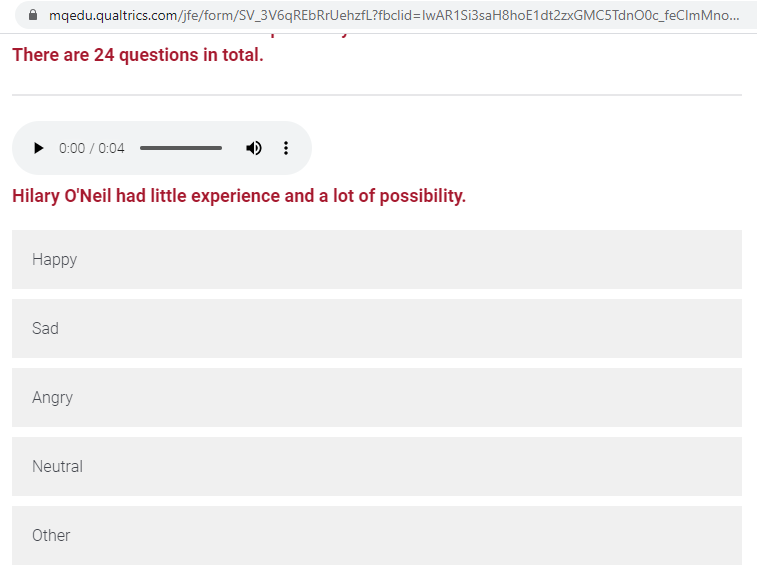
\includegraphics[width=7cm,height=9cm,keepaspectratio]{Images/Qualtrics_Survey.png}
        \caption{Sample Qualtrics survey question for emotion annotation}
        \label{fig:qualtrics_sample}
    \end{figure}
    
The emotion labels were collected from three annotators and the most common answer was used as the final label for the audio and its respective transcript. In case of no commonality in the answers, the group took it upon themselves to decide the final label of the observation which is still one of the answers by one of the annotators. The distribution of the emotions from the audio and transcript extracted from YouTube are shown in Figure \ref{fig:emo_YouTube}.
    
    \begin{figure}[H]
        \centering
        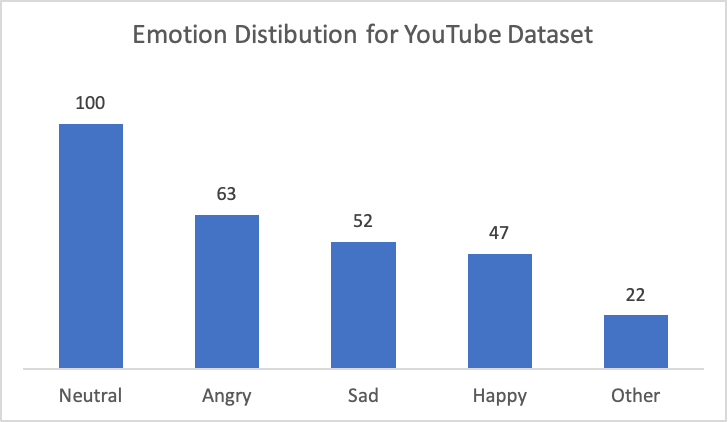
\includegraphics[width=8cm,height=12cm,keepaspectratio]{Images/emo_yt.png}
        \caption{Emotion distribution for data collected on YouTube}
        \label{fig:emo_YouTube}
    \end{figure}
    
The inter-annotator agreement was also calculated for the whole dataset and each individual video. Fleiss Kappa was utilised in the computation since the survey had answers from 3 different annotators. The results are displayed in Table \ref{Table_fleiss}.

    \begin{table}[H]
        \centering
        \begin{tabular}{|   c   c|}
        \hline
        Video & Fleiss Kappa \\
        \hline
        Dying Young Trailer & 0.40 \\
        Trailers of Top 5 Romance Movies & 0.45 \\
        UNTUCKED: Rupaul's Drag Race & 0.36 \\
        All videos & 0.44 \\
        \hline
        \end{tabular}
        \caption{Inter-annotator agreement for YouTube data}
        \label{Table_fleiss}
    \end{table}

The inter-annotator agreement for the individual videos ranges from 0.36 to 0.45 while the overall inter-annotator agreement is 0.44. This level would be considered weak to moderate agreement and makes the annotations less accurate. As a final note, keys were created for each audio-transcript-label pair to link the observations together.
\end{subs}

\begin{subs}
\subsection{Approach 2: Using an Existing Dataset from a Similar Research}
In this approach, the group did extensive research on previous studies or experiments that also tackled on a similar objective of predicting emotions using audio data. Most of the studies found also used the IEMOCAP dataset. An article from Towards Data Science titled Identifying Emotions from Voice using Transfer Learning\cite{towardsds} looked promising and used two audio datasets: The Ryerson Audio-Visual Database of Emotional Speech and Song (RAVDESS)\footnote{\url{https://zenodo.org/record/1188976\#.X6P26ZMzamk}} \cite{livingstone_steven_r_2018_1188976}and Toronto Emotional Speech Set (TESS)\footnote{\url{https://tspace.library.utoronto.ca/handle/1807/24487}} \cite{SP2/E8H2MF_2020}. Both datasets were recorded by voice actors in a controlled environment, i.e., minimal background noise. The RAVDESS dataset, however, only contains 2 transcripts that is uttered by 24 different actors portraying different emotions. Hence, the TESS data was picked for this approach.
\end{subs}

\begin{subs}
\subsubsection*{TESS Dataset Description}
This dataset was collected by the University of Toronto, Psychology Department in 2010. There were 200 target words spoken by two actresses (aged 26 and 64 years) and recordings were made portraying each of seven emotions: anger, disgust, fear, happiness, pleasant surprise, sadness, and neutral. The observations corresponding to the relevant emotions were then filtered for a total of 1,600 audio files (2 speakers, 200 transcripts and 4 emotions).
\end{subs}

\begin{subs}
\subsubsection*{Transcription Extraction}
The TESS data does not come with transcription, so the group had to extract them using Google Cloud Speech API which had 5.53\% word error rate. It was expected to have a very high speech-to-text conversion accuracy since the audio files were recorded in a controlled environment. 
\end{subs}

\begin{subs}
\subsubsection*{Emotion Labels}
The files are structured in a such a way that emotions can easily be extracted from each audio file. The amount of audio files are equally distributed among the four emotions with 400 observations each.

Similar to YouTube data, keys were created for each audio-transcript-label pair to link each observation in the TESS data.
\end{subs}

\begin{subs}
\subsection{Data Processing}
Since the newly constructed dataset from YouTube and TESS come in a new format, it had to be processed to fit the model’s input parameters. The first step was to replicate the processing of the raw IEMOCAP data to get an idea of what type of inputs are needed by the model. This was performed on both audio and text data. It took a big chunk of the group's time since they had to deal with Python package conflicts, e.g., some NLTK commands are unable to load properly in Python 2 environment. When all the issues were resolved, the processing pipeline in the research was applied to the newly constructed datasets.
\end{subs}

\begin{subs}
\subsubsection*{Text Processing}
Two versions of text processing was performed. The first one was similar to the processing in the research which was very minimal and typical of processing in text analysis. It only includes transforming the transcripts to lower case and tokenizing them to words. The second version included additional text processing, which includes removing non-alphanumeric characters and stop words, and retaining relevant keywords only, i.e., nouns, verbs, adjectives and adverbs. Both text files were filtered for transcriptions that have emotion labels in the four emotion categories only and converted into a numpy array. There were 262 transcriptions left on YouTube data.
\end{subs}

\begin{subs}
\subsubsection*{Audio Processing}
To process the audio data and extract the relevant features, the research used the openSMILE toolkit. This was the biggest challenge in processing the audio data since the team had to quickly familiarise themselves with the platform. Performing the installation and processing in Virtual Machine did not go well due to storage constraints. It was agreed to install the toolkit on Google Colaboratory as well as the local machines, as a backup.

The audio feature extraction derived MFCC and prosodic features. The MFCC feature set contains 39 features: 12 MFCC parameters (1-12) from the 26 Mel-frequency bands and log-energy parameters, 13 delta and 13 acceleration coefficients. The prosodic feature set contains 35 features such as F0 frequency, the voicing probability, and the loudness contours. These processing are both applied to YouTube and TESS datasets.

Similar filtering is done afterwards to retain the MFCC and prosodic features of observations that have the relevant emotion labels.
\end{subs}

\section{Results of New Data}
    The results of extending the research on YouTube and TESS datasets are shown side by side with the results published in the paper and the replication on the original data. Table \ref{Table_sec3.2} shows the retraining of the original data and the published results.  Table \ref{Table_sec5}, on the other hand, shows the accuracy results of the YouTube data alongside the results from the TESS data.
    
    \begin{table}[H]
        \centering
        \begin{tabular}{|   c   c   c |}
        \hline
        Model & YouTube Data & TESS Data \\
        \hline
        Text Only & 32.7\% & 25.0\% \\
        Audio Only & 23.5\% & 30.6\% \\
        Multimodal & 27.3\% & 34.9\% \\
        Multimodal-Attention & 23.9\% & 30.8\%\\
        \hline
        \end{tabular}
        \caption{New data replication accuracy}
        \label{Table_sec5}
    \end{table}
    
    As clearly shown, the evaluation on the new data resulted in accuracies way below the published results across the board. These results are best  shown in the barchart in Figure \ref{fig:barchart_results}.
    
    \begin{figure}[H]
        \centering
        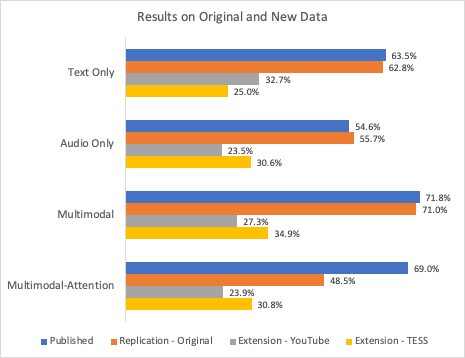
\includegraphics[width=10cm, height=8cm, keepaspectratio]{Images/replication_result.png}
        \caption{Replication on original data and extension on new data}
        \label{fig:barchart_results}
    \end{figure}
    
    The blue bar shows the benchmark published result in each of the models.  The orange bar is the result of the replication on the original IEMOCAP data. All results except MDREA seems consistent with the published results.\par
    
    The grey bar represents the results from the YouTube data whereas the yellow bar are for the TESS data.  In both cases, the models barely achieved 30\% accuracy.\par
    
    The accuracy results achieved during the extension of the research were short of the published results.  To the naked eye, this may ring bells of concern. Drilling further down, however, it should be recognised that there is a massive difference between the data used in the original training versus that used in this replication project. The techniques used here are completely different and the project is in fact an extension of the original model. For a maiden run of such new methodologies, this is in fact a good start and a good result at that.  Further fine-tuning will improve on these results.\par
    
\section{Summary and Reflections}
    Overall, this replication and extension project is deemed to have been successful given the limitations during the generation of the new data. The scores are in no doubt below the published results. However, the data used in the replication were very rudimentary and were not produced with the same level of sophistication as the original data. The low results here are just the initial results. It is still early days. Granted extra time, the replication team are confident that the techniques on generating new data can still be fine-tuned to hopefully end up with a higher accuracy result close to the published results. In addition, other factors may have contributed to the differences and may need to be reconsidered.
    
    \subsubsection*{Absence of pre-trained model}
        The source codes were made available but the pre-trained model was missing hence the need to execute the training phase the models.  It would have been more efficient had the model been available for at least three reasons - (1) elimination of the training time, (2) minimised chance of an introduced error and (3) established weights means more consistent accuracy.\par
    
        By rerunning the training source codes, it costed the replication team about 10 to 12 additional hours. It also forced the team to rethink how to save the pre-trained model. In running the MDREA model, there was also an unidentified discrepancy in the accuracy figure – a possible example of introduced error somewhere.\par
    
    \subsubsection*{OpenSMILE configurations tuned to IEMOCAP data}
        OpenSMILE gives the users opportunity to create their own configuration files, and use it in extracting features with openSMILE. In this research, modified configuration files were created and used by the authors of the original work in extracting audio and emotion features from the IEMOCAP audio data. These modified configuration files may be tuned in IEMOCAP audio data, which might be the cause of the big difference in accuracy of the original data results and new data results. The configuration that the authors made, can perform good feature extractions on an audio recorded in a controlled environment like the IEMOCAP and TESS data, and not that well on audio with noisy background like the YouTube data.\par
    
    \subsubsection*{Effect of TESS dataset variability}
        It was observed that in the TESS dataset, the transcripts have been shared between different emotions. The same transcripts have been spoken in different intonations which may have caused discrepancies in the prediction of labels especially those models utilising text data.\par
    
    \subsubsection*{Effect of background music}
        YouTube videos were used in this project. These spelled two issues.  Firstly, annotators may find that the tone of the background music affected how the emotions were labelled.\par
        
        A positive word spoken with a sad music tone made annotators label them as sad.\par

        Distortion of the audio sound is another issue. The original IEMOCAP dataset were collected in a controlled environment with potentially better acoustics. The YouTube videos in comparison have some noisy background.\par
        
    \subsubsection*{Annotation improvements}
        The annotation surveys have received only three responses.  A higher number of annotators would have improved the annotation accuracy. A high response will require a utility to pick the correct answer.  One transcript, for instance, has been annotated as neutral, angry, and sad by different annotators.  Which emotion will apply in these cases?  A possible algorithm fix could be to pick the modal response. Say for instance that a transcript has 20 responses with 5 neutral, 14 angry and 1 sad, pandas function \verb|db.mode()|, can label that transcript as angry.
        Additionally, Fleiss Kappa has been used to indicate inter-annotator agreement. With only three responses, the Fleiss Kappa resulted in a score of 0.44. This suggests a fair to moderate agreement \cite{fleisskappa} between the annotators which may denote inaccurate annotations and hence might explain the low accuracy score achieved in the YouTube dataset across all models.\par

\newpage
\printbibliography
%\bibliographystyle{plain}
%\bibliography{multi.bib}

\newpage
\section*{Appendix}
\begin{subappendices}
    \subsection*{Complete list of surveys used for YouTube data emotion annotation.}
    \begin{subs}
        \subsubsection*{Dying Young Trailer}
            \begin{itemize}
                \item \url{https://mqedu.qualtrics.com/jfe/form/SV_3V6qREbRrUehzfL}
            \end{itemize}
            
        \subsubsection*{Trailers of Top 5 romance movies of all time}
        \begin{itemize}
            \item \url{https://mqedu.qualtrics.com/jfe/form/SV_aWfIqIE47zNqQiF}
            \item \url{https://mqedu.qualtrics.com/jfe/form/SV_9zs3qKmWTmEXIaN}
            \item \url{https://mqedu.qualtrics.com/jfe/form/SV_2mJfhZUqAeBOHyd}
            \item \url{https://mqedu.qualtrics.com/jfe/form/SV_5gS1alMioRNID5j}
            \item \url{https://mqedu.qualtrics.com/jfe/form/SV_4YHTSBAAnPTWmeV}
            \item \url{https://mqedu.qualtrics.com/jfe/form/SV_6ETL75m3gZ8GneB}
            \item \url{https://mqedu.qualtrics.com/jfe/form/SV_4UsoeTpDaejmyvH}
            \item \url{https://mqedu.qualtrics.com/jfe/form/SV_0ddSfHUv29ljs3P}
            \item \url{https://mqedu.qualtrics.com/jfe/form/SV_egtQkblhurwcGoZ}
            \item \url{https://mqedu.qualtrics.com/jfe/form/SV_1Gp9SQeOXHhe2ot}
            \item \url{https://mqedu.qualtrics.com/jfe/form/SV_bwQNmDokIGzulQ9}
            \item \url{https://mqedu.qualtrics.com/jfe/form/SV_6hc6nkmrPOQYgyp}
            \item \url{https://mqedu.qualtrics.com/jfe/form/SV_diBPgwl6G0FWSbP}
            \item \url{https://mqedu.qualtrics.com/jfe/form/SV_54quaKRcyY3hBrL}
            \item \url{https://mqedu.qualtrics.com/jfe/form/SV_5dzcJEMHMPMpcuF}
            \item \url{https://mqedu.qualtrics.com/jfe/form/SV_1RAZxwNgXhj5QXP}
            \item \url{https://mqedu.qualtrics.com/jfe/form/SV_ekXULT5y7ucumQR}
        \end{itemize}
        
        \subsubsection*{UNTUCKED: Rupaul's Drag Race S09 E04}
        \begin{itemize}
            \item \url{https://mqedu.qualtrics.com/jfe/form/SV_82F4MKD2h4Chc8Z}
            \item \url{https://mqedu.qualtrics.com/jfe/form/SV_aicSb3q30AuU8YJ}
            \item \url{https://mqedu.qualtrics.com/jfe/form/SV_2cynAKMsqwGvQRD}
        \end{itemize}
    \end{subs}
\end{subappendices}
\end{document}